\chapter{Espaços e Funções Mensuráveis}

Nesta seção é apresentado um preambulo para a teoria medida.
Iniciaremos definindo \sigal para que possamos construir espaços mensuráveis.
Em seguida, abordaremos as funções mensurável.
Todas as definições e resultados aqui explorados tiveram como principais fontes \cite{elon}, \cite{bartle} e \cite{magalhaes}.

\section{O Conceito de \sigal}
Saber o que é uma \sigal e conseguir identificá-la em um espaço mensurável é fundamental para esta teoria.
Com isso, esta seção é dedicada para explorar definição, exemplos e propriedades sobre essa.
Vale ressaltar que é esperado que o leitor esteja familiarizado com a teoria elementar de conjuntos, bem como os conceitos principais de cálculo diferencial e integral.
Mesmo assim, em alguns momentos alguns conceitos e propriedades particulares são retomadas.

% Definição de Sigma álgebra
\begin{definition}
\label{def:sigma-algebra}

    Seja $X$ um conjunto não vazio. Uma família $\mathcal{C}$ de subconjuntos de $X$ é dita uma \sigal se as seguintes condições são atendidas:
    \begin{enumerate}[label*= (\roman*)]
        \item $\varnothing$ e $X$ são elementos de $\mathcal{C}$;     
        \item Se um elemento $A \in \mathcal{C}$, então $A^c \in \mathcal{C}$
        \footnote{Em todo o texto, $X^c$ significa o \textit{complementar do conjunto} $X$.};
        \item Se $(A_n)$ é uma sequência de elementos de $\mathcal{C}$, 
        então $\displaystyle \bigcup_{j = 1}^\infty A_j \in \mathcal{C}$.
    \end{enumerate}

\end{definition}

Um par ordenado $(X, \mathcal{C})$  constituído de um conjunto $X$ e uma \sigal sobre $X$ é chamado de  \textbf{espaço mensurável} . \index{espaço mensurável}
Além disso, cada elemento deste espaço é chamado de conjunto $\mathcal{C}-$mensurável.
Quando não houver confusão ou quando a \sigal estiver fixada, dizemos simplesmente que cada elemento é um conjunto mensurável.

\begin{remark}
	Em todo o texto, indicaremos por $I_n$ o conjunto dos $n$ primeiros números naturais. 
	Assim, $I_n = \{k \in \N; 1 \leq k \leq n\}$.
\end{remark}

% União finita de elemento da sigma algebra
\begin{proposition}
\label{prop:sigma-união-finita}
    Seja $\mathcal{C}$ uma \sigal de um conjunto $X$. Se $A_1, ..., A_n$ são todos elementos quaisquer de $\mathcal{C}$, então $\displaystyle \bigcup_{j = 1}^n A_j$ é um elemento de $\mathcal{C}$.
\end{proposition}
\begin{prova}
	Seja $A_1,\ldots, A_n$ elementos de $\cc$. 
	Construa uma sequência $(B_n)$ tal que $B_j = A_j$ para todo $j \in I_n$ e $A_{n + 1} = A_{n + 2} = \cdots = \varnothing$.
	Desta forma, pelo item \textit{(iii)} da definição de \sigal, temos que 
	$
	\displaystyle\bigcup_{j = 1}^\infty B_j = \bigcup_{j = 1}^n A_j
	$.
	Como $\displaystyle \bigcup_{j = 1}^\infty B_j \in \cc $, segue que 
	$\displaystyle \bigcup_{j = 1}^n A_j \in \cc $.
\end{prova}

%\begin{remark}
%	Às vezes, por praticidade, denotaremos a união enumerável infinita de uma família de elementos $(E_n)$ de uma \sigal $\cc$ como 
%	$\displaystyle \bigcup_{n \in \N} E_n$ ao invés de 
%	$\displaystyle \bigcup_{j = 1}^\infty E_n$.
%	A mesma convenção pode ser aplicada para interseção.
%\end{remark} 
% 
 
% Exemplos de Sigmas Algebras 
\begin{example}
    Seja $X = \{-1,0,-1\}$. Se considerarmos $\mathcal{C} = \{\varnothing, X, \{0\}, \{-1,1\}\}$, temos que $(X, \mathcal{C})$ é um espaço mensurável.
\end{example}

\begin{example}
\label{ex:sigma-trivial}
    Seja $X$ um conjunto qualquer.
    O conjunto $\mathcal{C}_1 = \{\varnothing, X\}$ é uma \sigal de $X$.
\end{example}

De fato, podemos observar que, nesse exemplo, todas as condições impostas na definição \ref{def:sigma-algebra} são atendidas de maneira trivial, pois 
$\varnothing$ e $X$ são todos os elementos de $\mathcal{C}_1$. 
Assim,  $(X, \mathcal{C}_1)$ é um espaço mensurável.
%
Perceba que a definição \ref{def:sigma-algebra} não nos diz que uma \sigal de um conjunto é única.
Realmente, não é. 
Assim, um conjunto pode gerar espaços mensuráveis diferentes a depender da \sigal adotada.
Para evidenciar essa percepção, observe o exemplo a seguir:

\begin{example}
	\label{ex:sigma-subconjuntos}
	Seja $X$ dado de maneira arbitrária conforme o exemplo anterior.
	Considere, agora, o conjunto $\mathcal{C}_2 = \{ A; \ A \subset X\}$, ou seja, o conjunto formado por todos os subconjuntos do conjunto $X$.
	%
	\footnote{O conjunto $\cc_2$ também é chamado de conjunto das partes de $X$ e, as vezes, é representado por $\mathcal{P}(X)$.}
\end{example}

Sabemos que $\varnothing \subset X$ e $X \subset X$. 
Assim, $\varnothing, X \in \mathcal{C}_2$. 
Se tomarmos um conjunto $A \subset \mathcal{C}_2$, então $A^c = X - A$ por definição.
Ou seja, $A^c$ é formado por elementos que estão todos em $X$ caracterizando-o um elemento de $\mathcal{C}_2$.
Da mesma forma, se tomarmos uma sequência $(A_j)$ de elementos de $\mathcal{C}_2$, a reunião 
$\displaystyle \bigcup_{j = 1}^\infty A_j$ é composta por elementos de $X$.
Logo,  $\displaystyle \bigcup_{j = 1}^\infty A_j \in \mathcal{C}_2$.
Com isso, $\mathcal{C}_2$ também é uma \sigal de $X$ e o par $(X, \mathcal{C}_2)$ é um espaço mensurável que, por sua vez, é diferente do espaço $(X,\mathcal{C}_1)$.


% Como todo estudo de matemática, após vermos definição e exemplos precisamos aprofundar-nos na natureza do objeto que estamos estudando.
% Partindo deste ponto, vamos dar início a uma sequencia de proposições que servirão como ferramenta para caracterizações futuras dos espaços mensuráveis.

Os exemplos apresentados acima são todos de conjuntos que são uma \sigal de um conjunto $X$ arbitrário.
Por definição, o conjunto $\mathcal{C}$ é composto de subconjuntos do conjunto $X$. 
Será que se construirmos $Z$ um conjunto que contenha $\varnothing$ e $X$ e outros subconjuntos do conjunto $X$ tomados aleatoriamente teremos $(X,Z)$ um espaço mensurável? A resposta é negativa e para convencê-lo disso, mostraremos o seguinte contra-exemplo.

%Contra Exemplo
\begin{counterexample}
    Seja $X = \{x,y,z\}$. O conjunto $\mathcal{C} = \{\varnothing, X, \{x\}, \{y\}, \{z\}\}$ não é uma \sigal de X.
\end{counterexample}

Sem dúvida, $\varnothing, X \in \mathcal{C}$. 
Entretanto, perceba que $\{x\} \in \mathcal{C}$, mas $\{x\}^c \notin \mathcal{C}$.
De fato, 
$$
\{x\}^c
=\{x,y,z\} 
-\{x\} 
= \{y,z\}.
$$
Entretanto, $\{y,z\} \notin \mathcal{C}$.
Assim, a segunda condição da definição \ref{def:sigma-algebra} não é satisfeita impossibilitando que $\mathcal{C}$ seja uma \sigal de $X$.
Com isso, podemos ver que uma \sigal não é construída de maneira tão trivial.
Entretanto, ás vezes, em matemática, é interessante conseguirmos induzir, em algum conjunto, uma propriedade que desejamos. 
A proposição adiante nos mostra como podemos induzir uma \sigal com um conjunto fixado não vazio em um conjunto.

% Assim, pode ser preciso construir uma \sigal em algum momento com um conjunto $A$ específico.
% A proposição adiante nos mostra como isso pode ser feito:

\begin{proposition}
\label{prop:sigma-complementar}
    Seja $X$ e $A$ dois conjuntos quaisquer com $A \neq \varnothing$.
    Se $A \subset X$, então o conjunto 
    $\mathcal{C}=\{\varnothing, X, A, A^c\}$ é uma \sigal de $X$.
\end{proposition}

\begin{prova}
    Perceba que as condições \textit{(i)} e \textit{(ii)} da definição \ref{def:sigma-algebra} são satisfeitas pela forma que o conjunto  $\mathcal{C}$ foi construído. Para verificar a última condição, basta perceber $A \cup A^c = X$. Assim, as sequências construídas terão comportamento análogo as do exemplo \ref{ex:sigma-subconjuntos}. Portanto, $\mathcal{C}$ é uma \sigal de $X$ para qualquer que seja $ \varnothing \neq A \subset X$.
\end{prova}

\begin{example}
    Considere $X = \N$. 
    Sejam $P =\{2k; \ k \in \N\}$ e $I = \{2k - 1;\ k \in \N\}$. 
    Como $P^c = I$, então $\mathcal{C} = \{\varnothing, \N, P, I\}$ é uma \sigal de $\N$ pela proposição anterior.
\end{example}

Observe que o conjunto $A$ que apresentamos na proposição \ref{prop:sigma-complementar} é um subconjunto não vazio do conjunto $X$ que fora tomado arbitrariamente. 
\footnote{Observe que se $A = \varnothing$, a \sigal é a mesma do exemplo \ref{ex:sigma-trivial}.}
Uma pergunta intuitiva é: se tomarmos um conjunto $A$ que não é subconjunto de $X$ o espaço $(X, \mathcal{C})$ continua sendo mensurável? A resposta é não.
Se o conjunto $A$ não for subconjunto de $X$ não temos como garantir a validade da condição \textit{(ii)}  da definição \ref{def:sigma-algebra}, pois  $A^c$ não é necessariamente um subconjunto de $X$ o que não permitiria os argumentos usados anteriormente na proposição \ref{prop:sigma-complementar}.
 
Dito isso, note que a definição \ref{def:sigma-algebra} e a proposição \ref{prop:sigma-união-finita} tratam apenas da união enumerável ou finita, respectivamente. 
Nosso interesse, agora, é investigar se conseguirmos propriedades análogas para a operação de interseção. 
Iniciaremos verificando o comportamento de interseção de elementos de uma \sigal com a proposição adiante.
% Propriedades de Interseção 

\begin{proposition}
\label{prop:interseção-elementos-sigmas}
    Seja $X$ um conjunto e $\mathcal{C}$ uma \sigal desse conjunto.
    Se $(A_j)$ é uma sequência  de conjuntos $\mathcal{C} $-mensuráveis, então $\displaystyle \bigcap_{j = 1}^\infty A_j$ é um elemento $\mathcal{C}$-mensurável.
\end{proposition}
\begin{prova}
    Se $A_j \in \mathcal{C}$ para todo $j \in \N$, então cada complementar $A_j^c \in \mathcal{C}$, pois $\mathcal{C}$ é $\sigma$-álgebra. 
    Assim, $(A_j^c)$ forma uma sequência de conjuntos $\mathcal{C}$-mensuráveis acarretando que 
    $\displaystyle \bigcup_{j = 1}^\infty A_j^c \in \mathcal{C}$. 
    Segue, pelas \textit{Leis de Morgan}
    \footnote{Caso não conheça consulte \supercite{elon}{p.26}}, que 
    $$
    \displaystyle \bigcup_{j = 1}^\infty A_j^c 
    = \left(\displaystyle \bigcap_{j = 1}^\infty A_j\right)^c
  	$$
	Logo, $\left(\displaystyle \bigcap_{j = 1}^\infty A_j\right)^c \in \mathcal{C}$ o que implica $\displaystyle \bigcap_{j = 1}^\infty A_j \in \mathcal{C}$. 
	Portanto, $\displaystyle \bigcap_{j = 1}^\infty A_j$ é um conjunto $\mathcal{C}$-mensurável.
\end{prova}

Considere a \sigal apresentada na proposição \ref{prop:sigma-complementar}. 
Qualquer outra \sigal $\mathcal{F}$ que tiver $A$ como elemento, conterá $\mathcal{C}$.
Assim, observamos que 
$$
\mathcal{C} = \displaystyle \bigcap_{\mathcal{F} \supset A} \mathcal{F}.
$$
Esta \sigal $\mathcal{C}$   definimos como a \textit{menor} \sigal gerada por $A$. \index{gerada por um conjunto}
%
\footnote{Lembre que a noção de \enquote{menor} aqui é trazida por meio da relação de ordem parcial gerada pela relação de inclusão entre conjuntos.}
%
Sabendo que a menor \sigal é gerada por meio de intersecções é natural questionarmos se a interseção entre \sigals ainda é uma \sigal de $X$.Para responderemos à esta pergunta com a proposição adiante.

%Interseção de Sigmas algebras
\begin{proposition}
\label{prop:interseção-2sigmas}
    Se $\mathcal{C}_1$ e $\mathcal{C}_2$ são duas \sigals de um conjunto $X$, então $\mathcal{C} = \mathcal{C}_1 \cap \mathcal{C}_2$ também é uma \sigal do conjunto $X$.
\end{proposition}

\begin{prova}
    Se $\mathcal{C}_1$ e $\mathcal{C}_2$ são \sigals de $X$, então ambos possuem $\varnothing$ e $X$ como elementos.
    Assim, $\varnothing$ e $X$ estão na intersecção $\mathcal{C}$.
    Além disso, se $A \in \mathcal{C}$, então $A \in \mathcal{C}_1$ e $A \in \mathcal{C}_2$. 
    Por serem ambas \sigals, $A^c \in \mathcal{C}$ e $A^c \in \mathcal{C}_2$.
    Ou seja, $A^c \in \mathcal{C}_1 \cap \mathcal{C}_2 = \mathcal{C}$.
    Por fim, se tomarmos uma sequência $(A_n)$ de elementos de $\mathcal{C}$, observamos que $A_j \in \mathcal{C}_1$ e $A_j \in \mathcal{C}_2$ para cada $j \in \N$.
    Assim, $\displaystyle \bigcup_{j = 1}^\infty A_j \in \mathcal{C}_1$ e 
    $\displaystyle \bigcup_{j = 1}^\infty A_j \in \mathcal{C}_2$ pela definição de \sigal.
    Logo, $\displaystyle \bigcup_{j = 1}^\infty A_j \in \mathcal{C}$.
    Com isso, $\mathcal{C}$ satisfaz todas as condições da definição \ref{def:sigma-algebra}. 
    Portanto, $\mathcal{C}$ é uma \sigal de $X$.
\end{prova}

\begin{proposition}
\label{prop:interseção-sigmas}
    Seja $(\mathcal{C}_j)$ uma sequência finita de $\mathcal{C}_j$-álgebras de um conjunto $X$, então 
    $\mathcal{C} = \displaystyle \bigcap_{j =1}^n\mathcal{C}_j$, com $n \geq 2$, também é uma \sigal do conjunto $X$.
    
\end{proposition}
\begin{prova}
    Provaremos esse resultado utilizando o método da indução finita sobre $n$.
    Se $n = 2$, o resultado é verificado imediatamente pela proposição \ref{prop:interseção-2sigmas}.
    Suponha que se verifique para algum $k \in \N$, isto é, $\displaystyle \bigcap_{j =1}^k\mathcal{C}_j$ é uma \sigal de $X$.
    Vamos checar para o sucessor de $k$.
    Ora, pela associatividade da interseção, vemos que 
    \begin{align*}
        \displaystyle \bigcap_{j =1}^{k+1}\mathcal{C}_j = \left(\displaystyle \bigcap_{j =1}^k\mathcal{C}_j\right) \cap \cc_{k+1}.
  	\end{align*}
	Denote $\displaystyle \bigcap_{j =1}^k\mathcal{C}_j = H$. 
	Sabemos por hipótese de indução que $H$  e $\cc_{k+1}$ são  \sigals de $X$. 
	Segue, pela base de indução, que $H \cap \cc_{k+1}$ é uma \sigal de $X$.
	Portanto, $\displaystyle \bigcap_{j =1}^{k+1}\mathcal{C}_j$ é uma \sigal de $X$ como queríamos.
\end{prova}

Note que há uma diferença gritante entre as proposições \ref{prop:interseção-elementos-sigmas} e \ref{prop:interseção-2sigmas}.
A primeira trata de conjuntos mensuráveis de uma \sigal e a outra refere-se à \sigals de um conjunto $X$.
Além disso, perceba que até aqui trabalhamos o conceito de \sigal de maneira abstrata sendo utilizada em um conjunto qualquer. 
Trataremos, agora, de uma \sigal extremamente importante e específica para o conjunto $\R$ dos números reais.

\begin{definition}
\label{def:algebra-borel}
    Seja $X = \R$. A Álgebra de Borel é a \sigal $\borel$ gerada por todos os intervalos abertos $(-\infty,x)$ com $ x  \in \R$. 
    Os elementos dessa \sigal são chamados de Borelianos.
    \index{Álgebra de Borel}

\end{definition}

Esta \sigal é extremamente relevante para os estudos de medida e integração e pode ser definida de várias formas diferentes, mas todas são equivalentes.
Isso quer dizer que $(-\infty, x)$ não é a única forma dos elementos de $\borel$. 
De fato, se  $(-\infty, x) \in \borel$, então $(-\infty, x)^c \in \borel$ só que $(-\infty, x)^c = [x, +\infty$).
Assim, poderíamos  definir  $\borel$ por meio de intervalos do tipo $[x, +\infty)$.
Em particular, poderíamos ter definido a $\borel$ por meio da \sigal gerada por intervalos do tipo $(a,b)$ com $a,b \in \R$. 

Antes de provamos este fato, observe que podemos decompor intervalos reais como a união de outros intervalos reais. 
Por exemplo, utilizando a reta real, podemos representar intervalo $(-\infty, b)$ da seguinte maneira\\

% Imagem da decomposição de intervalos.
\begin{figure}[h!]
	\centering
	\Caption{\label{fig:boreliano} Representação do intervalo $(-\infty, b)$ na reta real}	
	\UECEfig{}{
	    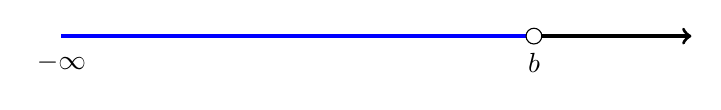
\begin{tikzpicture}
              % Eixo horizontal
              \draw[->, very thick] (-4,0) -- (4,0);
            
              % Linha vertical para representar x
              \draw[dashed] (2,-0.1) -- (2,0.1);
              % Rótulo para -∞
              \node[below] at (-4,-0.1) {$-\infty$};
              % Rótulo para x
              \node[below] at (2,-0.1) {$b$};
              % Desenhar o intervalo aberto (-∞, x)
              \draw[ultra thick, blue] (-4,0) -- (2,0);
              % Adicionar a bolinha aberta em x
              \draw[fill=white] (2,0) circle (0.1);
        \end{tikzpicture}
	}{
	    \Fonte{Elaborado pelo autor}
	}	
\end{figure}
Se tomarmos um $a \in \R$ fixo, com $a<b$, então a decomposição do intervalo $(-\infty, b)$ pode ser expressa por meio da união dos intervalos $(-\infty, a]$ e $(a,b)$, onde estão representados na figura a seguir pelas cores azul e vermelha respectivamente.\\
\begin{figure}[h!]
	\centering
	\Caption{\label{fig:boreliano-decomposto} Representação de uma decomposição do intervalo $(-\infty, b)$ na reta real}	
	\UECEfig{}{
        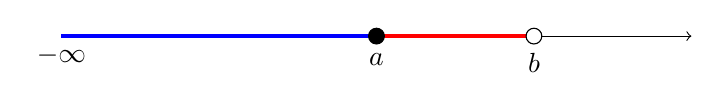
\begin{tikzpicture}
              % Eixo horizontal
              \draw[->] (-4,0) -- (4,0);
              % Linha vertical para representar x
              \draw[dashed] (2,-0.1) -- (2,0.1);
              % Rótulo para -∞
              \node[below] at (-4,0) {$-\infty$};
              % Rótulo para x
              \node[below] at (2,-0.1) {$b$};
                
              % Rótulo para a
              \node[below] at (0,-0.1) {$a$};
              
              % Desenhar o intervalo aberto (-∞, x)
              \draw[ultra thick, blue] (-4,0) -- (2,0);
            
              % Desenhar o intervalo aberto (a,b)
              \draw[very thick, red] (0,0) -- (2,0);
              
              % Adicionar a bolinha aberta em x
              \draw[fill=white] (2,0) circle (0.1);
              \draw[fill=black] (0,0) circle (0.1);
        \end{tikzpicture}
	}{
	    \Fonte{Elaborado pelo autor}
	}	
\end{figure}\\

Embora a decomposição de intervalos reais pela união de outros é extremamente relevante para mostrar a seguinte equivalência sobre a \sigal de Borel.\\
\begin{theorem}
\label{teo:equiv-borel}
    Uma \sigal é uma de Borel  se, e somente se, é gerada por intervalos do tipo $(a,b)$ com $a,b \in \R$.
\end{theorem}

\begin{prova}
   Suponha que $(\R,\borel)$ é um espaço mensurável. 
   Sejam $a$ e $b$ números reais, com $a<b$.
   Como $a - \dfrac{1}{n} \in \R$ para todo $n \in \N$, temos que o intervalo
   $\left(-\infty, a- \dfrac{1}{n}\right) \subset \R$ para todo $n \in \N$.
   Segue, pela proposição \ref{prop:interseção-elementos-sigmas}, que
   $\displaystyle \bigcap_{n = 1}^n \left(-\infty, a- \dfrac{1}{n}\right) \in \cc$.
   Com isso, afirmamos que a interseção de todos os intervalos $\left(-\infty, a - \dfrac{1}{n}\right)$ é igual ao intervalo $(-\infty, a]$.
   De fato,
   \begin{align*}
   		x \in \bigcap_{n \in \N} \left(-\infty, a - \dfrac{1}{n}\right)
   		\Leftrightarrow & x \in \left(-\infty, a - \dfrac{1}{n}\right), \ \forall n \in \N\\
   		\Leftrightarrow & x < a - \dfrac{1}{n}, \ \forall n \in \N\\
   		\Leftrightarrow & \dlim_{n \to \infty} x \leq \dlim_{n \to \infty} \left(a - \dfrac{1}{n}\right)\\
   		\Leftrightarrow & x \leq a\\
   		\Leftrightarrow & x \in (-\infty, a].
   \end{align*}
	Logo, $(-\infty, a] \in \borel$ acarretando que $(a, +\infty) = (-\infty, a]^c \in \borel$.
	Observe que podemos decompor $(-\infty, b) = (-\infty,a] \cup (a, b)$ enquanto que $(a, +\infty) = (a, b) \cup [b, +\infty)$.
	Desta forma, vemos que $(-\infty, b) \cap (a, +\infty) = (a,b)$. 
	Como $(-\infty, b)$ e $(a, +\infty)$ são elementos de $\borel$, segue pela proposição
	\ref{prop:interseção-elementos-sigmas} que $(a,b) \in \borel$.
	Com isso, $\borel$ pode ser gerada por intervalos do tipo $(a,b)$ com $a,b \in \R$.
   
	Suponha, reciprocamente, que $\mathcal{C}$ é uma \sigal de $\R$.
	Se $\cc$ é gerada por intervalos do tipo $(a,b)$ onde $a,b \in \R$, então
	os conjuntos $A_n = (-n, b)$ são todos elementos de $\mathcal{C}$ para qualquer $n \in \N$.
	Segue, pela definição \ref{def:sigma-algebra}, que 
	$\displaystyle \bigcup_{n = 1}^\infty (-n,b) \in \mathcal{C}$.
	Só que $\displaystyle \bigcup_{n = 1}^\infty (-n,b) = (-\infty, b)$.
	Com isso, os elementos de $\mathcal{C}$ são do tipo $(-\infty, b)$.
	Portanto, $\mathcal{C} = \borel$.

\end{prova}

\section{Funções Mensuráveis}


Agora que já estamos familiarizados com os conceitos de \sigal e espaços mensuráveis, vamos aplicar, sobre este espaço uma função e estudar seu comportamento.
\footnote{Em todo o texto função, aplicação e mapa são sinônimos.}
Iniciaremos tratando de funções à valores reais e estenderemos o conceito conforme haja necessidade.
Além disso, a partir de agora, fixemos que quando não houver menção contrária,  que $X$ será um conjunto qualquer diferente de $\varnothing$ e $\mathcal{C}$ será uma \sigal desse conjunto. 

\begin{definition}
	\label{def:mensurabilidade-funções-reais}
    Uma função $f: X \to \R $ é dita $\mathcal{C}$-mensurável se, para cada $\alpha \in \R$, o conjunto $\{x \in X;\ f(x) > \alpha\} \in \mathcal{C}$.
\end{definition}

% Exemplos de Funções mensuráveis

\begin{example}[Função Constante]
\label{ex:funcao-constante}
	Seja $K \in \R$ um número fixado. 
	A função $f: X \to \R$ definida por $f(x) = K$, para todo $x \in \R$  é $\cc$-mensurável.
\end{example}
Para mostrarmos este fato, precisamos analisar os casos de $\alpha$.
Assim
	\begin{enumerate}[label*= (\Roman*)]
		\item Se $\alpha \geq K$, então o conjunto $\{x \in X; f(x) > \alpha\} = \varnothing$ uma vez que não existe $x \in X$ tal que $f(x)= K > \alpha$.
		\item Se $\alpha < K$, então para todo $x \in X$, $f(x) > \alpha$.
		Logo, o conjunto $\{x \in X; f(x) > \alpha\} = X$.
	\end{enumerate}
Em todo caso, para todo $\alpha \in \R$, o conjunto  $\{x \in X;\ f(x) > \alpha\} \in \mathcal{C}$.
Portanto, a função constante $f$ é $\cc$-mensurável.
\begin{example}[Função Característica]
    Seja $(X, \mathcal{C})$ uma espaço mensurável e $A \in \mathcal{C}$.
    A função característica \footnote{As vezes também é chamada  função indicadora.} de $A$ 
    $\chi_A: X \to \{0,1\}$ definida por 
    $$\chi_A(x) =\left\{\begin{array}{cc}
         1, & \textrm{\ se \ } x \in A \\
         0, & \textrm{\ se \ } x \notin A
    \end{array}\right.
    $$
    É $\cc$-mensurável.
\end{example}

Para verificar se $X_A$ é $\cc$-mensurável precisamos, novamente, analisar os casos de $\alpha \in \R$.
	\begin{enumerate}[label*= (\Roman*)]
		\item Se $\alpha \geq 1$, observamos que $\{x \in X; \chi_A(x)>  \alpha\} = \varnothing$, pois não há $x \in X$ tal que $\chi_A(x) > 1$.  
		\item Se $ 0 <\alpha < 1$, então o conjunto $\{x \in X; \chi_A(x)>  \alpha\} = A$, pois apenas valores $x \in A$ tem suas imagens $\chi_A(x) = 1$ e consequentemente $\chi_A(x) \geq \alpha$.
		\item  se $\alpha \leq 0$, podemos notar que o conjunto $\{x \in X; \chi_A(x)>  \alpha\} = X$, pois para qualquer que seja $x \in X$, os valores $\chi_A(x) \geq 0$.
	\end{enumerate}
Em todo o caso, vemos que o conjunto $\{x \in X; \chi_A(x)>  \alpha\}$ é um elemento de $\mathcal{C}$, pois $\varnothing, X$ e $A$ são elementos de $\mathcal{C}$. Portanto, a função característica $\chi_A(x)$ é $\cc$-mensurável.
\begin{example}
\label{ex:função-continua-mensuravel}
    Considere o espaço mensurável $(\R, \borel)$. Toda função $f: \R \to \R$ contínua é Borel mensurável.
\end{example}
	Para mostrar a validade do exemplo acima, precisamos de resultados auxiliares que encontraremos em \cite{elon}.
	Um deles é a proposição abaixo.
\begin{proposition}
\label{cit:função-continua-mensuravel}
	Suponha que $f:X \to \R$ seja contínua em todos os pontos de $X$.
	Se $X \subset \R$ é um aberto
	\footnote{Em caso de dúvida sobre o que é um subconjunto $X$ de $\R$ aberto, consulte \supercite{elon}{p.164}.}, então o conjunto $A = \{a \in X;\ f(a)>k\}$ é um aberto (p.226).
\end{proposition}

	Note que o conjunto $\{x \in \R; f(x) > \alpha\} = (\alpha, +\infty)$.
	Logo, trata-se de um conjunto aberto.
	\footnote{Vide \supercite{elon}{p.164}.}
	Além disso, em \supercite{elon}{p.167}, encontramos o seguinte teorema:
	
	\begin{theorem}[Estrutura de abertos da reta]
		\label{teo:estrutura-abertos-reta}
		Todo subconjunto aberto $A \subset R$ se exprime, de modo único, como um reunião enumerável de intervalos abertos dois a dois disjuntos.
	\end{theorem}
	
	Segue disso que o
	$\{x \in \R; f(x) > \alpha\} = \displaystyle \bigcup_{j = 1}^\infty A_n$ onde cada $A_n$ é um intervalo aberto, ou seja $A_n \in \borel$ para todo $n \in \N$.
	Com isso, pela definição \ref{def:sigma-algebra}, o conjunto $\{x \in \R; f(x) > \alpha\} \in \borel$.
	Portanto, qualquer função contínua $f: \R \to \R$ é Borel mensurável.


    Lembre que ao apresentarmos a Álgebra de Borel (definição \ref{def:algebra-borel}), mostramos no teorema \ref{teo:equiv-borel} que há mais de uma maneira de definir os borelianos.
    Para uma função $f: X \to \R$ $\cc$-mensurável, também podemos definir uma função $\cc$-mensurável por meio de conjuntos diferentes conforme o seguinte teorema.

\begin{theorem}
\label{teo:equiv-funcoes-mensuraveis}
    Sendo $(X,\mathcal{C})$ um espaço mensurável, para uma função $f: X \to \R$ $\cc$-mensurável as seguintes afirmações são equivalentes:
    \begin{multicols}{2}
        
    \begin{enumerate}[label=(\alph*)]
        \item $\forall \ \alpha \in \R, \ A_\alpha =\{x \in X;\ f(x) > \alpha \} \in \mathcal{C}$;
        \item $\forall \ \alpha \in \R, \ B_\alpha =\{x \in X;\ f(x) \leq \alpha \} \in \mathcal{C}$;
        \item $\forall \ \alpha \in \R, \ C_\alpha =\{x \in X;\ f(x) \geq \alpha \} \in \mathcal{C}$;
        \item $\forall \ \alpha \in \R, \ D_\alpha =\{x \in X;\ f(x) < \alpha \} \in \mathcal{C}$.
    \end{enumerate}
     \end{multicols}

\end{theorem}

\begin{prova}
    Dividiremos esta demonstração em três partes. A estratégia será mostrar que a afirmação $(a)$ é equivalente à afirmação $(b)$; depois que a afirmação $(c)$ é equivalente à afirmação $(d)$ ; e por fim que a firmação $(a)$ ocorre se, e somente se, a afirmação $(c)$ ocorre. 
    \begin{enumerate}[label* = (\Roman*)]
        \item Suponha a validade da afirmação $(a)$. Se $A_\alpha \in \mathcal{C}$, então $A_\alpha^c \in \mathcal{C}$, pela definição de $\mathcal{C}$-álgebra.
    Perceba que 
    $$
    x \in A_\alpha^c \Leftrightarrow   x \notin A_\alpha\\
    \Leftrightarrow  x \in X \textrm{\ e \ } f(x) \leq \alpha, \forall\ \alpha \in \R
    \Leftrightarrow x \in B_\alpha    
	$$ Assim, um elemento está em $A_\alpha^c$ se, e somente se, está em $B_\alpha$. Segue que $A_\alpha^c = B_\alpha$. Logo, $B_\alpha$ é elemento de $\mathcal{C}$.
	\item Para mostrar a equivalência entre as afirmações $(c)$ e $(d)$ utilizamos um argumento totalmente análogo à parte $(I)$, pois se $x \notin C_\alpha$, então $f(x) < \alpha$ acarretando que $x \in D_\alpha$ e vice-versa.
	\item Suponha que $A_\alpha \in \mathcal{C}$. Tome a sequência $\left(A_{\alpha -\frac{1}{n}}\right)$. Claramente, cada $A_{\alpha - \frac{1}{n}}$ é um elemento de $\mathcal{C}$ por definição.
	Logo, pela proposição \ref{prop:interseção-elementos-sigmas}, a interseção $\displaystyle \bigcap_{n = 1}^\infty A_{\alpha -\frac{1}{n}} \in \mathcal{C}$. Além disso, note que 
\begin{align*}
    x \in \displaystyle \bigcap_{n = 1}^\infty A_{\alpha -\frac{1}{n}}
    \Leftrightarrow & x \in A_{\alpha - \frac{1}{n}}, \forall \ n \in \N\\
    \Leftrightarrow & f(x)> \alpha -\dfrac{1}{n},  \ \forall \ n \in \N\\
    \Leftrightarrow &\lim_{n \to \infty} f(x) \geq \lim_{n \to \infty} \left(\alpha - \dfrac{1}{n}\right)\\
    \Leftrightarrow & f(x) \geq \alpha \\
    \Leftrightarrow & x \in C_\alpha
\end{align*}
    \end{enumerate}
Desta forma, $C_\alpha = \displaystyle \bigcap_{n = 1}^\infty A_{\alpha -\frac{1}{n}} $. Logo $C_\alpha \in \mathcal{C}$ como queríamos.

Reciprocamente, suponha que $C_\alpha \in \mathcal{C}$. Tomemos a sequência $\left(C_{\alpha + \frac{1}{n}}\right)$.
Cada elemento $C_{\alpha +\frac{1}{n}} \in \mathcal{C}$ por definição.
Assim, pela definição de \sigal, 
$\displaystyle \bigcup_{n = 1}^\infty C_{\alpha +\frac{1}{n}} \in \mathcal{C}$. Com isso, temos que
\begin{align*}
    x \in \displaystyle \bigcup_{n = 1}^\infty C_{\alpha +\frac{1}{n}}
    \Leftrightarrow & x \in C_{\alpha + \frac{1}{n_0}}, \textrm{\ para algum  $n_0 \in \N$ }\\
    \Leftrightarrow & f(x)\geq \alpha +\dfrac{1}{n_0}\\
    \Leftrightarrow & f(x) > \alpha \\
    \Leftrightarrow & x \in A_\alpha
\end{align*}
Assim, $\displaystyle \bigcup_{n = 1}^\infty C_{\alpha +\frac{1}{n}} = A_\alpha$. Logo, $A_\alpha \in \mathcal{C}$.
Portanto, segue de $(I), (II)$ e $(III)$ que as afirmações $(a), (b), (c)$ e $(d)$ são todas equivalentes.


\end{prova}

% Aritmética de Funções mensuráveis
Perceba que mesmo na presença do teorema \ref{teo:equiv-funcoes-mensuraveis} acima, mostrar que uma função é mensurável é trabalhoso e repetitivo uma vez que, geralmente, é preciso verificar os casos de $\alpha$.
Com o intuito de otimizar a identificação de uma função mensurável, veremos o comportamento de operações aritméticas entre funções mensuráveis.

\begin{proposition}
\label{prop:aritmetica-uma-funcao}
Seja $f: X \to \R$ uma função real $\cc$-mensurável e $c \in \R$. Então as funções $cf$, $f^2$ e $|f|$ são $\cc$-mensuráveis. 
\end{proposition}

\begin{prova}
    \begin{enumerate}[label*=(\alph*)]
        \item Mostraremos que $cf$ é $\cc$-mensurável para todos os casos possíveis do número real $c \in \R$.
            \begin{enumerate}[label=(\roman*)]
                \item Se $c = 0$, então $c\cdot f(x) = 0, \ \forall \ x \in X$, ou seja, $cf$ se torna a função constante. Segue pelo exemplo \ref{ex:funcao-constante} que $cf$ é $\cc$-mensurável.
                
                \item Se $c>0$, então  dado $\alpha \in \R$, temos $cf(x) > \alpha \Leftrightarrow f(x) >\dfrac{\alpha}{c}$. 
                Logo, 
                $$
                \{x \in X; cf(x) > \alpha\} 
                = 
                \left\{x \in X; f(x) > \dfrac{\alpha}{c}\right\}
                $$
                    
                Isso ocorre para todo $\alpha$ e $f$ é $\cc$-mensurável, isto é, $\left\{x \in X; f(x) > \dfrac{\alpha}{c}\right\} \in \mathcal{C}$  . Logo, $cf$ é $\cc$-mensurável.
                
                \item Por fim, se $c < 0$, então existe um $z \in \R$ tal que $c = -z$.
                Assim, 
                $$cf(x) >\alpha \Leftrightarrow -zf(x) >\alpha \Leftrightarrow f(x) < -\dfrac{\alpha}{z}$$
                Assim, o conjunto $\{x \in X; cf(x) > \alpha \} = \left\{x \in X; f(x) < -\dfrac{\alpha}{z}\right\}$.
                Desta forma, o conjunto  $\left\{x \in X; f(x) < -\dfrac{\alpha}{z}\right\}  \in \mathcal{C}$ pelo  item $(d)$ do teorema \ref{teo:equiv-funcoes-mensuraveis}. Portanto,  $cf$ é $\cc$-mensurável em todos os casos de $c \in \R$.
            \end{enumerate}
            
        \item Para mostrar a mensurabilidade de $f^2$ é também necessário analisar os casos de $\alpha$.
            \begin{enumerate}[label = (\roman*)]
                \item Se $\alpha < 0$, então $\{x \in X; [f(x)]^2 > \alpha\} = X$, pois $[f(x)]^2 \geq 0$ para todo $x \in X$.
                
                \item Se $\alpha \geq 0$, então para todo $x \in X$ $[f(x)]^2 > \alpha \Leftrightarrow f(x) > \pm \sqrt{\alpha}$.
                Assim, um elemento 
                $x_0 \in \{x \in X; [f(x)]^2 > \alpha\}$ se, e somente se, $x_0 \in \{x \in X; f(x)> \sqrt{\alpha}\}$ ou \linebreak $x_0 \in \{x \in X; f(x)> -\sqrt{\alpha}\}$.
                Com isso, 
                
                $$\left\{x \in X; [f(x)]^2 > \alpha\right\} = \left\{x \in X; f(x)> \sqrt{\alpha}\right\}\cup \left\{x \in X; f(x)> -\sqrt{\alpha}\right\}$$
                
                Como $f$ é $\cc$-mensurável por hipótese, temos que $\{x \in X; f(x)> \sqrt{\alpha}\} \in \mathcal{C}$ e \linebreak $\{x \in X; f(x)> -\sqrt{\alpha}\} \in \mathcal{C}$.
                Desta forma, usando a definição de \sigal, obtemos que  $\{x \in X; f(x)> \sqrt{\alpha}\} \cup \{x \in X; f(x)> -\sqrt{\alpha}\} \in \mathcal{C}$. Consequentemente, 
                $\{x \in X; [f(x)]^2 > \alpha\} \in \mathcal{C}$ acarretando a mensurabilidade de $f^2$.
            \end{enumerate}
            
        \item Analogamente ao item anterior, se $\alpha < 0$, $\{x \in X; |f(x)| > \alpha\} = X$.
        Por outro lado, se $\alpha \geq 0$, vemos que 
        $\{x \in X; |f(x)| > \alpha\}=\{x \in X; f(x)> \alpha\} \cup \{x \in X; f(x)> -\alpha\}$.
        Assim, a mensurabilidade de $f$ acarreta na mensurabilidade de $|f|$ como desejávamos.
    \end{enumerate}
\end{prova}

% Exemplo de funções mensuráveis com aritmética
\begin{example}[Função Afim]
\label{ex:funcao-afim-mensuravel}
    Seja $a$ um número real diferente de zero. 
    A função $f: \R \to \R$ tal que $f(x) = ax$ é $\borel$-mensurável.
\end{example}
	
	De fato, pelo exemplo \ref{ex:função-continua-mensuravel} a função $x$ é $\borel$-mensurável, pois é contínua em $\R$.
	Segue pela proposição \ref{prop:aritmetica-uma-funcao} que a função $ax$ também é $\borel$-mensurável.
	Da maneira análoga, as funções $g,h: \R \to \R$ tais que $g(x) = x^2$ e $h(x) = |x|$ são $\borel$-mensuráveis. 
	A seguir veremos a mensurabilidade de combinações de funções mensuráveis.


\begin{proposition}
\label{prop:aritmetica-duas-funcoes}
    Sejam $f,g:X \to \R$. Se $f$ e $g$ são ambas $\cc$-mensuráveis, então as funções $f+g$ e $f\cdot g$ são também $\cc$-mensuráveis.
\end{proposition}

\begin{prova}
    Provaremos, primeiramente, que $f+g$ é $\cc$-mensurável.
    Ora, por hipótese, $f$ e $g$ são $\cc$-mensuráveis. 
    Assim, dado $r \in \Q$, os conjuntos $\{x \in X; f(x) > r\}$ e 
    $\{x \in X; g(x) > \alpha -r\}$ são ambos elementos de $\mathcal{C}$.
    Considere o conjunto  
    
    $$H_r = \{x \in X; f(x) > r\} \cap \{x \in X;\ g(x) > \alpha -r\}$$
    Isto é, o conjunto dos elementos $x \in X$ tal que $f(x) 
    > r$ e $g(x) >\alpha -r$ simultaneamente.
    Assim, afirmamos que $\{x \in X; (f+g)(x) > \alpha\} = \displaystyle \bigcup_{r \in \Q} H_r$. Com efeito, as seguintes equivalências ocorrem para um elemento $a \in X$ tomado arbitrariamente
        \begin{align*}
            a \in \{x \in X; (f+g)(x) > \alpha\} 
            \Leftrightarrow  & (f+g)(a) >\alpha \\
            \Leftrightarrow & f(a) +g(a) > \alpha \\
            \Leftrightarrow & f(a) + g(a) > \alpha -r + r\ \textrm{para } \ r \in \Q\\
            \Leftrightarrow & f(a) > r \textrm{\ e\ } g(a) > \alpha -r\ \textrm{para  } \ r \in \Q\\
            \Leftrightarrow & a \in \{x \in X; f(x) > r\} \textrm{\ e\ } a \in \{x \in X; f(x) > \alpha - r\}\  \textrm{para  } \ r \in \Q\\
            \Leftrightarrow & a \in \{x \in X; f(x) > r\} \cap \{x \in X; f(x) > \alpha - r\}\  \textrm{para  }  r \in \Q\\
            \Leftrightarrow & a \in H_r,\ \textrm{para  } \ r \in \Q\\
            \Leftrightarrow &a \in \bigcup_{r \in \Q} H_r.
        \end{align*}
    
    Concluindo que a afirmação é verdadeira. 
    Além disso, para cada $r \in \Q$, o conjunto $H_r$ é um elemento de $\mathcal{C}$, pois é  a interseção de dois elementos de $\mathcal{C}$ (proposição \ref{prop:interseção-elementos-sigmas}).
    Note também que, pela definição de $\mathcal{C}$, a coleção $\displaystyle \bigcup_{r \in \Q} H_r$ é um elemento de $\mathcal{C}$, pois $\Q$ é enumerável
    \footnote{Em caso de dúvida, vide \supercite{elon}{p.51}.}.
    Segue que $f+g$ é $\cc$-mensurável.

    Para mostrar que $fg$ é mensurável basta notar que é a combinação de outras funções $\cc$-mensuráveis.
    De fato, dado $x \in X$, temos
	    \begin{align*}
	        4(fg)(x) 
	        =& \ 2(fg)(x) +  2(fg)(x)\\
	        =& \ [f(x)]^2 - [f(x)]^2 + 2f(x)g(x) + [g(x)]^2 - [g(x)]^2 + 2f(x)g(x)\\
	        =& \ \left([f(x)]^2 + 2f(x)g(x) + [g(x)]^2\right)  - \left([g(x)]^2 - 2f(x)g(x) + [f(x)]^2\right)\\
	        =& \ (f(x) +g(x))^2 - (f(x) - g(x))^2\\
	        =& \ [(f+g)(x)]^2 - [(f-g)(x)]^2.
	    \end{align*}
    Desta maneira, $fg = \dfrac{1}{4}\left[(f+g)^2 - (f-g)^2\right]$. Segue pela proposição \ref{prop:aritmetica-uma-funcao} e a primeira parte desta demonstração que $fg$ é $\cc$-mensurável.
\end{prova}

\begin{example}[Função Polinomial]
\label{ex:funcao-polinomial-mensuravel}
    A função  $f:\R \to \R$ definida por $f(x) = \displaystyle \sum_{j = 0}^n a_jx^j$ com cada $a_j \in \R$ é $\borel$-mensurável.
\end{example}
   
    Com efeito, note que  $f(x) = a_nx^n + a_{n-1}x^{n-1} + \cdots + a_1x +a_0$.
	Pelo exemplo \ref{ex:funcao-afim-mensuravel} cada função $f_j:\R \to \R$ definida por  $f_j(x) = a_jx^j$ é $\borel$-mensurável.
	Além disso, pela proposição \ref{prop:aritmetica-duas-funcoes} a soma de funções mensuráveis é mensurável.
	Segue que $f(x) = \displaystyle\sum_{j = 0}^n a_jx^j$ é uma função $\borel$-mensurável.

\begin{definition}
	\label{def:parte-positiva e negativa}
    Seja $f: X \to \R$ uma função real. Dizemos que a \textbf{parte positiva} da função $f$ é a função $f^+: X \to \R$ definida por $f^+(x) = \sup\{f(x), 0\}$.
    Semelhantemente, chamamos de a \textbf{parte negativa} da função $f$, a função $f^-: X \to \R$ definida por $f^-(x) = \sup\{-f(x), 0\}$.
    \footnote{Em caso de dúvidas sobre o supremo de um conjunto real, vide \supercite{elon}{p.75}.}
\end{definition}

É possível  que a definição de parte positiva e negativa de funções fique um pouco abstrata em um primeiro contato. 
Numa tentativa de esclarecer ao máximo, daremos o seguinte exemplo:
\begin{example}
    Seja $f: \R^* \to \R$ definida por $f(x) =\dfrac{|x|}{x}$. 
    Então $f^+(x) = 1$ e $f^-(x) = -1$.
\end{example}

De fato, ao tomarmos um elemento real $x< 0$, vemos que sua imagem $f(x) < 0$ sendo $f(x) = \dfrac{-x}{x} = -1$.
Se $x>0$, então $f(x) =\dfrac{x}{x} = 1$. 
Assim, $f^+ = \sup\{f(x), 0\} = 1$ enquanto que $f^- = \sup\{-f(x), 0\} = -1$.
Neste caso, podemos perceber, ao olhar para a imagem \ref{fig: Gráfico da Função f(x) =|x|/x} a seguir que tanto a parte positiva quanto a parte negativa da função $f$ acima apresentada são ambas funções constantes.\\

    \begin{figure}[h!]
	\centering
	\Caption{\label{fig: Gráfico da Função f(x) =|x|/x} Gráfico da Função $f(x) =\dfrac{|x|}{x}$}	
	\UECEfig{}{
	    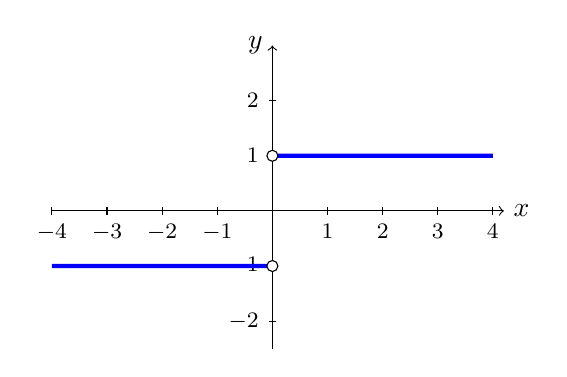
\begin{tikzpicture}[scale=0.7]
	    	% Eixos
	    	\draw[->] (-4,0) -- (4.2,0) node[right] {$x$};
	    	\draw[->] (0,-2.5) -- (0, 3) node[left] {$y$};
	    	% Rótulos
	    	\foreach \i in {-4,-3,-2,-1,1,2,3,4}{
	    		\draw (\i,2pt)--(\i, -2pt) node[below]{{\footnotesize $\i$}};
	    	}
	    	\foreach \i in {-2,-1,1,2}{
	    		\draw (2pt,\i)--(-2pt,\i) node[left]{{\footnotesize $\i$}};
	    	}
                
            \draw[domain=-4:-0.1,ultra thick,variable=\x,blue] plot ({\x},{abs(\x)/\x});
            \draw[domain=0.1:4,ultra thick,variable=\x,blue] plot ({\x},{abs(\x)/\x});
        
            \draw[fill=white] (0,1) circle (0.1);
            \draw[fill=white] (0,-1) circle (0.1);
        
            \end{tikzpicture}
	}{
	    \Fonte{Elaborado pelo autor}
	}	
    \end{figure}    

Por serem constantes, já vimos que são mensuráveis.
Mas e a função $f(x) =\dfrac{|x|}{x}$? Será que é mensurável?
A resposta é sim e para mostrarmos isso precisaremos de alguns resultados auxiliares. 
    \begin{lemma}
    \label{lem:decomposicao-da-funcao-em-partes-positiva-negativa}
        Seja $f: X \to \R$ uma função real. Então $f = f^+ - f^-$ e $|f| = f^+ + f^-$.
    \end{lemma}
    \begin{prova}
            Para provar que $f = f^+ - f^-$, devemos avaliar os casos de $f(x)$. 
            Logo, se $f(x) \geq 0$, então $f^+(x) = \sup\{f(x), 0\} = f(x)$ e $f^-(x) = \sup\{-f(x), 0\} = 0$, pois $f(x) \geq 0 \Rightarrow  - f(x) \leq~0$.
            Disso, $f^+(x) - f^-(x) = f(x) - 0 = f(x)$, ou seja, $(f^+ - f^-)(x) = f(x), \ \forall x \in X$.
            Caso $f(x) <~0$, então $- f(x) > 0$. 
            Com isso,  $\sup\{f(x), 0\} = 0$ e $\sup\{-f(x), 0\} = -f(x)$.
            Desta forma vemos que
            $f^+(x) - f^-(x) = 0 - (-f(x)) = f(x)$.
            Em todo caso, $f = f^+ - f^-$.

            Analogamente, se $f(x) \geq 0$, então  $\sup\{f(x), 0\} = f(x)$ e $\sup\{-f(x), 0\} = 0$.
            Assim, $f^+(x) + f^-(x) = f(x)$.
            Caso, $f(x) < 0$, então $ - f(x) > 0$.
            Com isso, obtemos $\sup\{f(x), 0\} = 0$ e $\sup\{-f(x), 0\} = -f(x)$.
            Logo, $f^+(x) + f^-(x) = -f(x)$.
            Desta forma, 
            $$
            (f^+ + f^-)(x) = \max\{f(x), -f(x)\} = |f(x)|.
            $$
            Portanto, $f^+ + f^- = |f|$.
    \end{prova}

Observe que o lema \ref{lem:decomposicao-da-funcao-em-partes-positiva-negativa} nos dá a forma das funções $f^+$ e $f^-$ de maneira implicita.
De fato, somando as duas expressões membro a membro vemos que 
$$f + |f| = (f^+ + f^+) - (f^- + f^-) = 2f^+$$
Assim, podemos expressar $f^+ = \dfrac{|f| + f}{2}$.
De modo semelhante, pode-se subtrair membro a membro e obter a expressão $f^- = \dfrac{|f| - f}{2}$. 
Isso demonstra o lema adiante:

    \begin{lemma}
    \label{prop:identidades-das-partes-das-funcoes}
        Se $f: X \to \R$ é uma função real, então $f^+ = \dfrac{|f| + f}{2}$ e $f^- = \dfrac{|f| - f}{2}$.
    \end{lemma}
Com isso, podemos responder à indagação anterior por meio do seguinte teorema:
    \begin{theorem}
        Uma função $f: X \to \R$ é $\cc$-mensurável se, e somente se, suas partes negativa e positiva são ambas $\cc$-mensuráveis. 
    \end{theorem}

    \begin{prova}
        Suponha que $f$ seja $\cc$-mensurável.
        Pela proposição \ref{prop:aritmetica-uma-funcao} vemos que a função $|f|$ é $\cc$-mensurável e pelo lema \ref{prop:identidades-das-partes-das-funcoes} as funções $f^+ = \dfrac{1}{2}(|f| + f)$ e $f^+ = \dfrac{1}{2}(|f| - f)$ também são $\cc$-mensuráveis.
        Desta forma, as funções $f^+$ e $f^-$ são combinações aritméticas de funções $\cc$-mensuráveis.
        Segue pela proposição \ref{prop:aritmetica-duas-funcoes} que $f^+$ e $f^-$ são $\cc$-mensuráveis.
        Reciprocamente, supondo que $f^+$ e $f^-$ são mensuráveis, temos pelo lema \ref{lem:decomposicao-da-funcao-em-partes-positiva-negativa} que
        $f = f^+ - f^-$. Segue, novamente pela proposição \ref{prop:aritmetica-duas-funcoes}, que $f$ é $\cc$-mensurável. 
    \end{prova}

Uma vez que foram apresentadas as definições de \sigal, espaços mensuráveis e funções mensuráveis; nosso alicerce está totalmente consolidado para que possamos entender o que é uma medida medida sem muita dificuldade.
Isso faremos na seção seguinte

    % \begin{example}
    %         Seja $f: \R \to \R$ definida por  $f(x) = (\cos x, \seno x)$.
    %         Ao analisarmos o gráfico de $f$, podemos observar que $f$ é uma circunferência de raio 1 centrada na origem conforme está ilustrada na figura abaixo
    %         \begin{figure}[h!]
    %         	\centering
    %         	\Caption{\label{fig:grafico-da-curva-circulo} Gráfico da curva $f(x) = (\cos x, \sin x)$}	
    %         	\UECEfig{}{
    %         	    \begin{tikzpicture}[scale=1.5]
    %                         % Eixos cartesianos
    %                         \draw[->] (-1.25,0) -- (2,0) ;
    %                         \draw[->] (0,-1.25) -- (0,1.75) ;
    %                         % Rótulos dos eixos
                            
    %                         \node at (1.1,-0.15) {$1$};
    %                         \node at (-0.15,1.15) {$1$};
    %                         % \foreach \x in {-1,1}
    %                         %   \draw (\x,0.05) -- (\x,-0.05) node[below right] {$\x$};
    %                         % \foreach \y in {-1,1}
    %                         %   \draw (0.05,\y) -- (-0.05,\y) node[left] {$\y$};
                            
    %                         % Gráfico da função
    %                         \draw[domain=0:2*pi,samples=100,thick,blue] plot ({cos(\x r)},{sin(\x r)});
    %                         % Legenda
    %                         \node[blue] at (1.2,1.2) {$f(x) = (\cos x, \sin x)$};
    %                     \end{tikzpicture}
    %         	}{
    %         	    \Fonte{Elaborado pelo autor}
    %         	}	
    %         \end{figure}
    %     Assim, $f^+= \sqrt{1 - x^2}$ enquanto que $f^- = - \sqrt{1 - x^2}$.
        
    % \end{example}
    
%%%%%%%%% ESPAÇOS MENSURÁVEIS
\section{Os Espaços de Funções Mensuráveis}
    Vimos até aqui é como identificar espaços e funções mensuráveis.
    As vezes, teremos conjuntos "muito grandes" que podem ser medidos, mas sua medida não poderá ser expressa por um número real.
    Para solucionar este problema, apresentaremos um novo sistema numérico.

    \begin{definition}
    \label{def:reta-estendida}
        A coleção $\xreta$ que consiste de $\R \cup \{-\infty, +\infty\}$ é chamada de \textbf{Sistema Estendido de Números Reais}.
    \end{definition}

    Este sistema é necessário por vários motivos que serão apresentados ao longo do texto. 
    Um deles, por exemplo, é a conveniência em dizer que o comprimento da Reta Real $\R$ é $+\infty$.
    Embora estejamos "adicionando" os símbolos $\pm \infty$ à reta real, vale a ressalva de que eles não são números.
    Com isso, $\xreta$ não é fechado para operações de $\R$ tais como $(+\infty) + (-\infty)$ que nem definido é.
    Dito isso, para $x \in \R$, as operações dos símbolos $+\infty$ e $-\infty$ são:
    \begin{multicols}{2}
        \begin{itemize}
            \item $(+ \infty) + (+ \infty)  = + \infty$;
            \item $x + (+ \infty) = (+ \infty) + x = + \infty$;
            \item $(- \infty) + (- \infty)  = - \infty$;
            \item $x + (- \infty) = (- \infty) + x = - \infty$;
            \item $(+ \infty)\cdot (+ \infty) =  +\infty $;
            \item $(- \infty)\cdot (- \infty) =  +\infty $;
            \item $(+ \infty)\cdot (- \infty) =  -\infty $;
            \item $(- \infty)\cdot (+ \infty) =  -\infty $.
        \end{itemize}
    \end{multicols}
    Na multiplicação, dependendo do número real, a operação diferencia-se.
    Assim, podemos ter
    \begin{multicols}{2}
    $$
    x \cdot (+\infty) = (+\infty) \cdot x =
    \left\{\begin{array}{cc}
          +\infty, & \ \textrm{se } x > 0\\
          0, & \ \textrm{se } x = 0\\
          - \infty, & \textrm{se } x < 0
    \end{array}\right.
    $$
    
    $$
    x \cdot (-\infty) = (-\infty) \cdot x =
    \left\{\begin{array}{cc}
          -\infty, & \ \textrm{se } x > 0\\
          0, & \ \textrm{se } x = 0\\
          + \infty, & \textrm{se } x < 0
    \end{array}\right.
    $$  
    \end{multicols}

    Neste novo contexto de números reais a \sigal de Borel não é mais válida uma vez que a definição \ref{def:algebra-borel} não inclui $+\infty$ nem $-\infty$.
    Com isso, considere $\xreta$.
    Tomando um conjunto arbitrário $E \in \borel$, com $\varnothing \neq E$, defina $E_1 = E \cup \{-\infty\}, E_2 = E \cup \{+\infty\}$ e $E_3 = E \cup \{-\infty, +\infty\}$. 
    Desta forma, o conjunto $\overline{\borel} = \displaystyle \bigcup_{E \in \borel} \{E, E_1, E_2, E_3\}$ é uma \sigal de $\xreta$. Com efeito, se $E \in \borel$, então é um intervalo aberto conforme o teorema \ref{teo:equiv-borel}.
    Assim, $E_1, E_2, E_3$ e $E_4$ serão intervalos do tipo $[-\infty,x)$ ou $(x, +\infty]$ que são elementos de $\borel$ acrescidos de $+\infty$ ou $-\infty$. 
    Deste modo, é fácil verificar que se um elemento $A \in \xborel$, então $A^c \in \xborel$.
    Além disso, a união enumerável é, no máximo, o intervalo $[-\infty,+\infty]$ que é exatamente $\xreta$.
    Desta forma, $\xborel$ é uma \sigal de $\xreta$.

    \begin{definition}
    \label{def:algebra-borel-estendida}
        A \sigal $\overline{\borel} = \displaystyle \bigcup_{E \in \borel} \{E, E_1, E_2, E_3\}$ do conjunto $\xreta$ é chamada de Álgebra de Borel Estendida. 
    \end{definition}

    Uma vez que estamos familiarizados com os conceitos de funções de valores reais mensuráveis, estamos prontos para estender este conceito para o conjunto $\xreta$.

    \begin{definition}
    \label{def:familia-funcoes-mensuraveis}
        Sendo $(X, \mathcal{C})$ um espaço mensurável, uma função de valores reais estendidos $f: X \to \xreta$ é dita $\mathcal{C}$-mensurável caso o conjunto
        $\{x \in X; f(x) > \alpha\} \in \mathcal{C}$ para qualquer que seja $\alpha \in \R$. 
    \end{definition}

	Denotaremos a família de todas as funções de valores reais estendidos de $X$ que são $\mathcal{C}$-mensuráveis por $M(X, \mathcal{C})$.
    \begin{proposition}
    \label{prop:identidade-intersecao-mais-infinito}
        Se $f \in \menfus$, então $\{x \in X; f(x) = +\infty\} = \displaystyle \bigcap_{n = 1}^\infty \{x \in X; f(x) > n\}$.
    \end{proposition}

    \begin{prova}
        Tome, de modo arbitrário, um elemento $a \in X$. 
        Assim, 
        \begin{align*}
            a \in \bigcap_{n = 1}^\infty \{x \in X; f(x) > n\} 
            \Leftrightarrow & a \in \{x \in X; f(x) > n\}, \ \forall n \in \N\\
            \Leftrightarrow & \forall n \in \N,\ f(a) > n\\
            \Leftrightarrow & \dlim_{n \to \infty} f(a) \geq \dlim_{n \to \infty} n\\
            \Leftrightarrow & f(a) \geq +\infty.  
        \end{align*}
    Como estamos trabalhando com $\xreta$, não existe elemento $x > +\infty$.
    Logo, o único elemento possível para $f(a)$ é $+\infty$.
    Assim, tudo isso ocorre se, e somente se, o elemento $a \in \{x \in X; f(x) = +\infty\}$ como queríamos.
    Além disso, note que cada $\{x \in X; f(x) > n\} \in \mathcal{C}$.
    Segue, pela proposição \ref{prop:interseção-elementos-sigmas}, que $\displaystyle \bigcap_{n = 1}^\infty \{x \in X; f(x) > n\} \in \mathcal{C}$ acarretando que $\{x \in X; f(x) = +\infty\} \in \mathcal{C}$. 
    \end{prova}

    \begin{proposition}
    \label{prop:identidade-união-menos-infinito}
        Se $f \in \menfus$, então $\{x \in X; f(x) = -\infty\} = \displaystyle \left(\bigcup_{n = 1}^\infty \{x \in X; f(x) > - n\}\right)^c$.
    \end{proposition}
	%
    \begin{prova}
        Analogamente à proposição \ref{prop:identidade-intersecao-mais-infinito} tomemos $a \in X$. 
        Segue que 
        \begin{align*}
            a \in \left(\bigcup_{n = 1}^\infty \{x \in X; f(x) > - n\}\right)^c
            \Leftrightarrow & a \in \bigcap_{n = 1}^\infty \left(\{x \in X; f(x) > - n\}\right)^c\\
            \Leftrightarrow & \forall \ n \in \N, a \in \left(\{x \in X; f(x) > - n\}\right)^c\\
            \Leftrightarrow & \forall \ n \in \N, a \notin \{x \in X; f(x) > - n\}\\
            \Leftrightarrow & \forall \ n \in \N, a \in \{x \in X; f(x) \leq - n\}\\
            \Leftrightarrow & \forall \ n \in \N, f(a) \leq - n\\
            \Leftrightarrow & \lim_{n \to \infty} f(a) \leq \lim_{n \to \infty} (- n)\\            
            \Leftrightarrow & f(a) \leq -\infty\\            
            \Leftrightarrow & f(a) = -\infty\\            
            \Leftrightarrow & a \in \{x \in X; f(x) = -\infty\}            
        \end{align*}
        
    Ora, cada $\{x \in X; f(x) > - n\} \in \mathcal{C}$.
    Assim, por definição de \sigal, temos que $ \displaystyle\bigcup_{n = 1}^\infty \{x \in X; f(x) > - n\} \in \mathcal{C}$ e também 
    $\displaystyle\left(\bigcup_{n = 1}^\infty \{x \in X; f(x) > - n\}\right)^c \in \mathcal{C}$.
    Concluímos disso que $\{x \in X; f(x) = -\infty\} \in \mathcal{C}$ como queríamos provar. 
    \end{prova}

    \begin{theorem}
    \label{teo:condição-de-mensurabilidade}
        Um função de valores reais estendidos $f: X \to \xreta$ é $\cc$-mensurável se, e somente se, os conjuntos 
        $A = \{ x \in X; f(x) = +\infty\}$ e $B = \{x \in X; f(x) = -\infty\}$
		 são elementos de $\mathcal{C}$ e a função $h: X \to \R$ definida por
		 
		 $$
		 h(x) = \left\{\begin{array}{cc}
		     f(x), & \textrm{\ se } x \notin A\cup B  \\
		      0,& \textrm{\ se } x \in A\cup B
		 \end{array}\right.
		 $$
		 é $\cc$-mensurável.
	 \end{theorem}
\begin{prova}
    Suponha que $f \in \menfus$. 
    Logo, pelas proposições \ref{prop:identidade-intersecao-mais-infinito} e \ref{prop:identidade-união-menos-infinito}, os conjuntos $A$ e $B$ são elementos de $\mathcal{C}$.
    Assim, tome $\alpha \in \R$ com $\alpha \geq 0$, então os elementos de $\{x \in X; h(x) > \alpha\}$ são os elementos de $\{x \in X; f(x) > \alpha\}$ que não estão em $A$, pois $h$ tem contradomínio $\R$.
    $A \in \cc \Rightarrow A^c \in \cc$. 
    Com isso, 
    $$
    \{x \in X; h(x) > \alpha\} = A^c\cap \{x \in X; f(x) > \alpha\} \in \cc
    $$
    Segue, pela proposição \ref{prop:interseção-elementos-sigmas} que $\{x \in X; h(x) > \alpha\} \in \cc$, ou seja, $h$ é $\cc$-mensurável.
    Caso, $\alpha < 0$, então os elementos de $\{x \in X; h(x) > \alpha\} = \{x \in  X ; f(x) > \alpha\} \cup B $, pois $h(x) = 0$ para $x \in A \cup B$.
    Desta forma $h$ é $\cc$-mensurável.

    Por outro lado, se supormos que $A$ e $B$ são elementos de $\mathcal{C}$ e $h$ é $\cc$-mensurável, então
    $$\{x \in X; f(x) > \alpha\} = \{x \in  X ; h(x) > \alpha\} \cup A $$
    quando $\alpha \geq 0$, e 
    $$\{x \in X; f(x) > \alpha\} = \{x \in  X ; h(x) > \alpha\} - B $$
    quando  $\alpha < 0$ por motivos análogos à primeira parte da demonstração.
    Portanto, $f$ é uma função $\cc$-mensurável como desejávamos.
\end{prova}

Como consequência do teorema \ref{prop:aritmetica-uma-funcao} e o teorema \ref{teo:condição-de-mensurabilidade} obtemos, imediatamente, que se $ f \in M(X,\mathcal{C})$, então as funções $cf, f^2, |f|, f^+$ e $f^-$ também são elementos de $M(X, \mathcal{C})$.
Entretanto, um resultado análogo à proposição \ref{prop:aritmetica-duas-funcoes} não possível em $\xreta$.
Isso acontece por que em $\xreta$ a operação de adição não é bem definida.
Então caso $f(x) = +\infty$ e $g(x) = -\infty$ para algum $x \in \R$ a adição
$f(x) + g(x)$ não é realizada.
Por outro lado, a função $fg$ é $\cc$-mensurável se $f$ e $g$ forem ambas $\cc$-mensuráveis.
Para mostrar isso, precisamos do seguinte teorema

\begin{theorem}
\label{teo:mensurabilidade-sequencia-funcoes-mensuraveis}
	Seja $(f_n)$ uma sequência de elementos de $\menfus$ e defina as funções
	$$f(x) = \inf f_n(x),\  
	F(x) = \sup f_n(x),\  
	f^*(x) = \lim\inf f_n(x),\   
	F^*(x) = \lim\sup f_n(x).$$
	Então as funções $f, f^*, F$ e $F^*$ são elementos de $\menfus$.
\end{theorem}
\begin{prova}
	Como $(f_n)$ é uma sequência de funções $\cc$-mensuráveis e $f = \inf f_n$, afirmamos que $\{x \in ; f(x) \geq \alpha\} = \displaystyle \bigcap_{n = 1}^\infty \{x \in X; f_n(x) \geq \alpha\}$.
	De fato, tomemos um elemento $h \in X$.
	Assim, 
		\begin{align*}
			h \in \bigcap_{n = 1}^\infty \{x \in X; f_n(x) \geq \alpha\} \Leftrightarrow	&
			h \in \{x \in X; f_n(x) \geq \alpha\}\ \forall n \in \N\\
			\Leftrightarrow	&	
			f_n(h) \geq \alpha\ \forall n \in \N\\
			\Leftrightarrow	&	
			\inf_{n \in \N}f_n(h) \geq \inf_{n \in \N}\alpha\ \forall n \in \N\\
			\Leftrightarrow	&	
			f(h) \geq \alpha\ \forall n \in \N\\
			\Leftrightarrow	&
			h \in \{x \in X; f(x) \geq \alpha\}
		\end{align*}
	Como cada $\{x \in X; f_n(x) \geq \alpha\}$ é $\cc$-mensurável, segue pela proposição \ref{prop:interseção-elementos-sigmas} que o conjunto $\{x \in X; f(x) \geq \alpha\} \in \cc$ para todo $\alpha \in \R$.
	Desta forma, $f$ é $\cc$-mensurável.
	
	Observe, também, que $\{x \in X; F(x) >\alpha\} = \displaystyle \bigcup_{n = 1}^\infty \{x \in X; f_(x) >\alpha\}$.
	Com efeito, para $h \in X$ 
	\begin{align*}
		h \in \bigcup_{n = 1}^\infty \{x \in X; f_n(x) > \alpha\} \Leftrightarrow	&
		\exists\ k \in \N \textrm{tal que\ } h \in \{x \in X; f_k(x) > \alpha\}\\
		\Leftrightarrow	&	
		f_k(h) > \alpha,\ \forall \alpha \in \R\\
		\Leftrightarrow	&	
		F(x) \geq f_k(h) > \alpha,\ \forall \alpha \in \R\\
		\Leftrightarrow	&	
		F(x) > \alpha,\ \forall \alpha \in \R\\
		\Leftrightarrow	&
		h \in \{x \in X; F(x) > \alpha\}
	\end{align*}
	Assim, concluímos que $f$ e $F$ são $\cc$-mensuráveis. 
	Note que a mensurabilidade de $f^*$ e $F^*$ vem de $f$ e $F$ uma vez que
	$$
	f^*(x) = \sup_{n \geq 1} \left\{\inf_{m \geq n} f_m(x)\right\}
	\textrm{\ e\ }
	F^*(x) = \inf_{n \geq 1} \left\{\sup_{m \geq n} f_m(x)\right\}
	$$
\end{prova}

\begin{corollary}
	\label{cor:convergencia-de-uma-sequencia-mensuravel}
	Se $(f_n)$ é uma sequência em $\menfus$ que converge para $f$ em $X$, então
	$f$ também está em $\menfus$.
\end{corollary}
\begin{prova}
	Ora, por hipótese $\displaystyle f(x) = \lim_{n \to +\infty} f_n(x)$.
	Só que $\displaystyle \lim_{n \to +\infty} f_n(x) = \lim_{n \in \N} \inf f_n(x)$.
	Segue que $\displaystyle f(x) = \lim_{n \in \N} \inf f_n(x)$ que, por sua vez, é $\cc$-mensurável pelo teorema anterior.
\end{prova}

% Parte final do Capítulo - Truncamento
\begin{definition}[Truncamento de uma função mensurável]
	Seja $f$ uma função em $\menfus$ e $A > 0$.
	Definimos o truncamento $f_A$ da função $f$ por
	$$ f_A(x) =
	\left\{\begin{array}{cc}
		f(x), & \textrm{se\ } |f(x)| \leq A \\
		A, & \textrm{se\ } f(x) > A \\
		-A, & \textrm{se\ } f(x) < A 
	\end{array}\right.
	$$
\end{definition}

% Exemplos de Truncamento

\begin{example}
	Seja $f \in \menfus$ tal que $f(x) = x^2-2$.
	Então o truncamento $f_2$ é representado, graficamente, como
	\begin{figure}[h!]
		\centering
		\Caption{\label{fig:representação do truncamento da função f(x) = x^2-2} representação do truncamento $f_2$ da função $f(x) = x^2-2$} 
		\UECEfig{}{
			\begin{tikzpicture}[scale=0.5]
				% Defina o intervalo x
				\def\xmin{-3}
				\def\xmax{3}
%				
%				% Desenhe a função f(x)
%				\draw[domain=\xmin+0.4:\xmax-0.4, smooth, samples=100, blue] plot (\x, {\x*\x -2});
				
				% Desenhando a função f_2
				\draw[domain=2:4.5, thick, samples=100, red] plot (\x, {2});
				\draw[domain=-4.5:-2, thick, samples=100, red] plot (\x, {2});
				\draw[domain=-2:2, thick, samples=100, red] plot (\x, {\x*\x -2});
				
				% Adicione rótulos aos eixos
				\draw[->] (\xmin-2,0) -- (\xmax+2,0) node[right] {$x$};
				\draw[->] (0,\xmin-1) -- (0,\xmax+2.5) node[above] {$y$};
				
                % Rótulos
				\foreach \i in {-4,-3,-2,-1,1,2,3,4}{
					\draw (\i,2pt)--(\i, -2pt) node[below]{{\footnotesize $\i$}};
				}
				
				\foreach \i in {1,2,3,4,5}{
					\draw (2pt,\i)--(-2pt, \i) node[left]{{\footnotesize $\i$}};
				}
			\end{tikzpicture}
		}{
			\Fonte{Elaborado pelo autor}		}   
	\end{figure}
	
\end{example}

	Observe que a figura \ref{fig:representação do truncamento da função f(x) = x^2-2} mostra que o truncamento $f_2$ efetua uma espécie de \enquote{limitação} da função $f$ pela constante $2$.

\begin{proposition}
	\label{prop:truncamento-mensurável}
	Seja $A$ um número real maior que zero.
	Se $f$ é uma função em $\menfus$, então $f_A$ é uma função $\cc$-mensurável.
\end{proposition}
\begin{prova}
	De fato, se os elementos $x \in X$ são tais que $A \leq f(x) \leq A$, então $f_A(x) = f(x)$.
	Logo $f_A$ é $\cc$-mensurável, pois $f$ o é.
	Caso esses elementos sejam tais que $f(x) > A$ ou $f(x) <A$ a função $f_A$ é constante.
	Segue pela proposição \ref{ex:funcao-constante} que $f_A$ é um elemento de $\menfus$.
\end{prova}

Retornemos para a mensurabilidade do produto de duas funções com valores reais estendidos.
Sejam $f,g \in \menfus$. 
Tomemos duas sequências $(f_n)$ e $(g_m)$ tais que para cada $k \in \N$, $f_k$ e $g_k$ são truncamentos de $f$ e $g$, respectivamente.
Ou seja, 
	$$ g_m(x) =
		\left\{\begin{array}{cc}
			g(x), & \textrm{se\ } |g(x)| \leq m \\
			n, & \textrm{se\ } g(x) > m \\
			-n, & \textrm{se\ } g(x) < m 
		\end{array}\right.	
	$$
e $f_n$ é definida de modo similar.
Pela proposição \ref{prop:truncamento-mensurável}, $f_n$ e $g_m$ são $\cc$-mensuráveis para cada $n$ e $m$ números naturais.
Assim, pela proposição \ref{prop:aritmetica-duas-funcoes} $f_ng_m$ também é $\cc$-mensurável para quaisquer $n, m \in \N$.
Como o truncamento de uma função $f$ causa uma \enquote{limitação} na função $f$ se tomarmos $n$ grande suficiente o truncamento $f_n$ tende a se aproximar da função $f$.
Assim, para $x \in X$
$$
\lim_{n \to +\infty} \left(f_n(x)g_m(x)\right) = f(x)g_m(x) 
$$
Segue pelo corolário \ref{cor:convergencia-de-uma-sequencia-mensuravel} que 
$fg_m \in \menfus$. Com isso, temos que para $x \in X$
$$
\lim_{m \to +\infty} \left(f(x)g_m(x)\right) 
= f(x)g(x) = (fg)(x)
$$
Segue, pelo mesmo corolário, que $fg \in \menfus$.

Nos tratamos da mensurabilidade de funções reais apenas.
Em alguns casos, é necessário trabalhar com mensurabilidade de uma forma mais abstrata, como na teoria de probabilidades, por exemplo.
Para encerrar esta subseção apresentaremos a definição abstrata de mensurabilidade de uma função.

\begin{definition}
	\label{def:mensurabilidade-abstrata}
	Sejam $(X, \cc)$ e $(Y,\mathcal{F})$ dois espaços mensuráveis.
	Dizemos que uma função $\phi:(X, \cc)\to (Y,\mathcal{F})$ é dita mensurável se o conjunto $f^{-1}(E) = \{x \in X; f(x)\in E\} \in \cc$ para todo conjunto $E \in \mathcal{F}$. 
\end{definition}

Embora essa definição pareça ser totalmente distinta da definição \ref{def:mensurabilidade-funções-reais}, as duas são equivalentes no caso particular de $Y = \R$ e $\mathcal{F} = \borel$ conforme demonstrado a seguir.

\begin{proposition}
	Seja $(X, \cc)$ um espaço mensurável e $f$ uma função.
	Então $f$ é $\cc$-mensurável se, e somente se. $f^{-1}(E) \in \cc$ para todo boreliano $E$. 
\end{proposition}
\begin{prova}
	Suponha $f$ uma função $\cc$-mensurável. 
	Sabemos pela definição \ref{def:algebra-borel} que os elementos da álgebra de Borel são do tipo $(-\infty,x)$ com $x \in \R$.
	Assim, dado arbitrariamente $\alpha \in \R$ temos que
	$$
	f^{-1}(-\infty, \alpha)
	=\{x \in X; f(x) \in (-\infty, \alpha)\}
	=\{x \in X; f(x) \leq \alpha\}
	\footnote{$f^{-1}(-\infty, \alpha)$ indica a pré imagem de $(-\infty, \alpha)$.}
	$$
	Como $f$ é $\cc$-mensurável segue pelo teorema \ref{teo:equiv-funcoes-mensuraveis} que $f^{-1}(-\infty, \alpha) \in \cc$.
	Reciprocamente se 
	$f^{-1}(-\infty, \alpha) \in \cc$ para qualquer $\alpha$ concluímos, imediatamente, que $\{x \in X; f(x) < \alpha\} \in \cc$ para todo $\alpha \in \R$.
	Portanto, $f$ é $\cc$-mensurável.
\end{prova}
%%%%%%%%%% Espaços de Medida

\section{Espaços de Medida}

Nas subseções anteriores, nós trabalhos com conjuntos e com funções mensuráveis, isto é, que podem ser medidas de alguma forma.
Nesta subseção, nos preocuparemos em definir e trabalhar com funções de um espaço mensurável $(X, \mathcal{C})$ que daremos o nome de "medida".
Tais funções são induzidas pela nossa concepção de comprimento, área, volume, etc.
Dito isso, para trabalhamos com medidas primeiro retomaremos alguns resutlados sobre sequência de conjuntos.

\begin{definition}
\label{def:sequência-crescente-decrescente-de-conjuntos}
    Uma sequência de conjuntos $(A_n)$ é dita \textbf{crescente} se $A_n \subseteq A_{n+1}$ para todo $n \in \N$.
    Caso tenhamos $A_n \supseteq A_{n+1}$ para todo $n \in \N$, dizemos que a sequência  de conjuntos é \textbf{decrescente}.
\end{definition}

\begin{proposition}
\label{prop:sequencia-crescente-conjuntos-resultado-A_n}
Seja $(E_n)$ uma sequência crescente de conjuntos. Se $(A_n)$ é tal que $A_1 = E_1$ e $A_n = E_n - E_{n -1}$ para todo $n > 1$, então:
\begin{enumerate}[label* = (\roman*)]
    \item $A_n$ é uma sequência disjunta;
        \footnote{Lembre que uma sequência disjunta significa que $A_i \cap A_j = \varnothing$ para todo $i \neq j$}
    \item $E_n = \displaystyle \bigcup_{j = 1}^n A_n$;
    \item $\displaystyle \bigcup_{j = 1}^\infty E_n = \displaystyle \bigcup_{j = 1}^\infty A_n$;
\end{enumerate}
\end{proposition}

\begin{prova}
    Para provar $(a)$ precisamos mostrar que para todo $n,m \in \N$ se $m \neq n$, então $A_n \cap A_m = \varnothing$.
    Lembre que $A - B = A\cap B^c$ para quaisquer conjuntos $A$ e $B$.
    Desta forma, como a interseção entre conjuntos é associativa e comutativa temos que
    \begin{align*}
        A_m\cap A_n =& (E_m - E_{m -1}) \cap (E_n - E_{n -1})\\
        =& (E_m \cap E_{m -1}^c) \cap (E_n \cap E_{n -1}^c)\\
        =& (E_m \cap E_n) \cap ( E_{m -1}^c\cap E_{n -1}^c)\\
        =& (E_m \cap E_n) \cap \left( E_{m -1}\cup E_{n -1}\right)^c\\
    \end{align*}
    Com isso, se $m > n$, então $E_n \subseteq E_m$ e $E_{n-1} \subseteq E_{m-1}$, pois $(E_n)$ é uma sequência crescente.
    Além disso, $E_m^c \subseteq E_{m -1}^c$ e $E_m \cap E_m^c = \varnothing$.
    Segue que
    $$
    (E_m \cap E_n) \cap \left( E_{m -1}\cup E_{n -1}\right)^c =
    (E_m) \cap E_{m -1}^c = 
    \varnothing
    $$
    Caso tenhamos $m < n$ temos $E_m \subseteq E_n$ e $E_{m-1} \subseteq E_{n-1}$.
    Segue analogamente que 
    $$
    (E_m \cap E_n) \cap \left( E_{m -1}\cup E_{n -1}\right)^c =
    (E_n) \cap E_{n -1}^c = 
    \varnothing
    $$
    Em todo caso, $A_m \cap A_n = \varnothing$ para todo $m \neq n$.

    Provaremos o item $(b)$ por indução sobre $n$.
    Como $(E_n)$ é crescente, temos que $E_1 \subseteq E_2$.
    Com isso, temos que 
        \begin{align*}
            \bigcup_{j = 1}^2 A_j = A_1 \cup A_2= & E_1 \cup (E_2 - E_1)\\
            = & E_1 \cup (E_2 \cap E_1^c)\\
            = & (E_1 \cup E_2) \cap (E_1 \cup E_1^c)\\
            = & (E_1 \cup E_2) \cap \mathcal{C}\\
            = & (E_1 \cap E_2)
            = E_2  
        \end{align*}
    Suponha que exista um $k \in \N$ tal que $\displaystyle \bigcup_{j = 1}^k A_j = E_k$.
    Mostraremos que $\displaystyle \bigcup_{j = 1}^{k+1} A_j = E_{k +1}$ também é verdadeira.
    Com efeito, 
    \begin{align*}
        \bigcup_{j = 1}^{k+1} A_j =& \left(\bigcup_{j = 1}^{k} A_j\right) \cup A_{k+1}\\
        =& E_k \cup A_{k +1}\\
        =& E_k \cup (E_k - E_{k+1})\\
        =& E_k \cap E_{k+1}\\
        =& E_{k+1}\\
    \end{align*}
    Segue, pelo método da indução finita, que $\displaystyle \bigcup_{j = 1}^n A_j = E_n\ \forall n \in \N$.

    Por fim, $(c)$ é um resultado imediato, pois $ x \in \displaystyle \bigcup_{j = 1}^\infty E_j$ se, e somente se, 
    existe um $n_0 \in \N$ tal que $x \in E_{n_0}$. 
    Pelo item $(b)$, isso só ocorre se $x \in \displaystyle \bigcup_{j = 1}^{n_0}A_j$.
    Mas isso é equivalente à dizer que existe um $k$ com $1\leq k\leq n_0$ tal que $x \in A_k$.
    Como $k \in \N$ isso acontece se, e somente se, $x \in A_k$ para algum $k \in \N$.
    Portanto $x \in \displaystyle \bigcup_{j = 1}^\infty A_j$.
\end{prova}

\begin{proposition}
\label{prop:sequencia-decrescente-conjuntos-resultado-A_n}
Seja $(F_n)$ uma sequência decrescente de conjuntos. 
Se $(E_n)$ é tal que $E_n = F_1 - F_n$ para todo $n \in \N$, então $(E_n)$ é crescente e 
$\displaystyle \bigcup_{j = 1}^\infty E_n = \displaystyle F_1 - \bigcup_{j = 1}^\infty F_n$.
\end{proposition}

\begin{prova}
    Queremos mostrar que $(E_n)$ é crescente, isto é, $E_n \subseteq E_{n+1}$ para todo $n \in \N$.
    Tome $x \in E_n$. Logo, $x \in F_1$ e $x \notin F_n$, por construção.
    Como $(F_n)$ é decrescente, $F_{n} \supseteq F_{n+1}$. 
    Assim, $x \notin F_n \Rightarrow x \notin F_{n+1}$.
    Com isso, $x \in F_1$ e $x \notin F_{n+1}$.
    Segue que $x \in E_{n+1}$ e que $E_n \subseteq E_{n+1}$ para qualquer $n \in \N$ como queríamos.
    Além disso, um elemento $a \in \displaystyle \bigcup_{n \in \N} E_n$ se, e somente se,
    $a \in \displaystyle \bigcup_{n \in \N} (F_1 - F_n)$.
    Isso é equivalente a dizer que existe um $n_0 \in \N$ tal que $a \in F_1 - F_{n_0}$.
    Correspondentemente, $ a \in F_1$ e existe um $n_0 \in \N$ tal que $x \notin F_{n_0}$.
    Isso só ocorre se $x \in F_1$, mas $x \notin \displaystyle \bigcup_{n \in \N} F_n$.
    Portanto, $\displaystyle \bigcup_{j = 1}^\infty E_n = \displaystyle F_1 - \bigcup_{j = 1}^\infty F_n$.
\end{prova}

\begin{definition}
\label{def:medida}
    Uma medida é uma função $\mu: (X, \mathcal{C}) \to \xreta$ tal que satisfaz as seguintes condições:
    \begin{enumerate}[label* = (\roman*)]
        \item $\mu(\varnothing) = 0$;
        \item $\mu(E) \geq 0, \ \forall A \in \mathcal{C}$;
        \item Se $(A_n)$ é uma sequência disjunta de elementos de  $\mathcal{C}$, então 
        $\displaystyle\mu\left(\bigcup_{n = 1}^\infty A_n\right) = \sum_{n = 1}^\infty\mu(A_n)$.
        
    \end{enumerate}
\end{definition}

Ou seja uma medida é uma função não negativa que é contavelmente aditiva.
Além disso, o valor de $\mu$ pode ser igual à $+\infty$ para algum conjunto $A \in \mathcal{C}$.
Quando temos que $\mu(E) < +\infty$ para qualquer que seja o conjunto $E \in \mathcal{C}$, dizemos que temos uma medida finita.

\begin{definition}
	\label{def:espaço-de-medida}
	Dizemos que uma tripla ordenada $(X, \mathcal{C}, \mu)$ constituída por um conjunto $X$, uma \sigal $\mathcal{C}$ desse conjunto e uma medida $\mu$ sobre o espaço mensurável $(X, \mathcal{C})$ é um espaço de medida.
\end{definition}


% Exemplos de medida

\begin{example}
    Seja $X$ um conjunto e $\mathcal{C}$ a sigma álgebra formada por todos os subconjunto de $X$.    
    Defina $\mu_1, \mu_2:\mathcal{C} \to \xreta$ pondo $\mu_1(A) = 0$ para qualquer  $A \in \mathcal{C}$ e 
    $\mu_2$ é  pondo 

$$\mu_2(A) = \left\{\begin{array}{cc}
0, & \textrm{\ se \ } A = \varnothing \\
+\infty,& \textrm{\ se \ } A \neq \varnothing
\end{array}\right.$$
Sendo definidas dessa forma, as funções $\mu_1$ e $\mu_2$ são medidas.
\end{example}

De fato, em ambas as condições \textit{(i)} e \textit{(ii)} são trivialmente satisfeitas.
Para a condição \textit{(iii)}, temos que qualquer sequência disjunta $(A_n)$ acarretará que

$$\mu_1\left(\bigcup_{n = 1}^\infty A_n\right) = 0 = \sum_{n = 1}^\infty 0 = \sum_{n = 1}^\infty \mu_1(A_n) $$
Para $\mu_2$ temos dois casos possíveis.
Se  $\displaystyle \bigcup_{n = 1}^\infty A_n  = \varnothing$, então $\mu_2\left(\displaystyle \bigcup_{n = 1}^\infty A_n\right) = 0$. Entretanto isso ocorre somente se $A_j = \varnothing$ para todo $j \in \N$.
Logo, 

$$\sum_{n = 1}^\infty \mu_2(A_n) = \sum_{n = 1}^\infty \mu_2(\varnothing) = \sum_{n = 1}^\infty 0 = 0$$
Caso $\displaystyle \bigcup_{n = 1}^\infty A_n  \neq  \varnothing$, conseguimos observar que os termos da sequência $(A_n)$ só podem ser de dois tipos ou $A_j = 0$ ou $A_j = +\infty$ para algum $j \in \N$. Com isso,  $\mu_2\left(\displaystyle \bigcup_{n = 1}^\infty A_n\right) = +\infty$.

Ademais, na soma $\displaystyle \sum_{n = 1}^\infty \mu_2(A_n)$ só teremos soma dos termos $0 + (+ \infty)$ ou $(+\infty) + (+\infty)$.
Desta forma, $\displaystyle \sum_{n = 1}^\infty \mu_2(A_n) = \sum_{n = 1}^\infty \mu_2(A_n) = +\infty$.
Portanto $\mu_1$ e $\mu_2$ são medidas.

% Probabilidade
\begin{example}[Probabilidade]
	Seja $(\Omega, \cc)$ um espaço mensurável.
	A função $\mathcal{P}:\cc \to [0,1]$ é dita uma probabilidade se satisfaz as propriedades:
	\begin{enumerate}[label* =(K\arabic*)]
		\item $\mathcal{P}(\Omega) = 1$;
		\item $\mathcal{P}(A) \geq 0,\ \forall A \in \cc$;
		\item Se $(A_n)$ é uma sequência disjunta de elementos de  $\mathcal{C}$, então 
		$\displaystyle\mathcal{P}\left(\bigcup_{n = 1}^\infty A_n\right) = \sum_{n = 1}^\infty\mathcal{P}(A_n)$.
		\footnote{As propriedades \textit{K1, K2} e \textit{K3} são chamadas de \textit{Axiomas de Kolmogorov}}
	\end{enumerate}
\end{example}

Observe que as condições da \textit{(ii)} e \textit{(iii)} da definição \ref{def:medida} são satisfeitas por definição da função de probabilidade.
Resta provar que $\mathcal{P}(\varnothing) = 0$.
Assim, com o auxilio das propriedades \textit{(K1)} e \textit{(K3)}, segue que 
$$
\pp(\Omega)
= 
\pp(\Omega \cup \varnothing)
= 
\pp(\Omega) + \pp(\varnothing)
\Rightarrow
\pp(\Omega)
= 
\pp(\Omega) + \pp(\varnothing)
$$
Logo, $\pp(\varnothing) = 0$. 
Portanto a função probabilidade é uma medida.
Neste caso, o espaço de medida $(\Omega, \cc, \pp)$ é chamado de espaço de probabilidades.
Além disso, uma função $\cc$-mensurável pela definição \ref{def:mensurabilidade-abstrata} em um espaço de probabilidades é chamada de variável aleatória.

% Unidade de Medida Concentrada em p
\begin{example}[Unidade de Medida Concentrada em $p$]
\label{ex:medida-concentrada-em-p}
    Seja $(X, \mathcal{C})$ um espaço mensurável tal como no exemplo $a$ e $p$ um elemento de $X$.
    Defina $\mu: \mathcal{C} \to \xreta$  como sendo


$$\mu(A) = \left\{\begin{array}{cc}
0, & \textrm{\ se \ } p \notin A \\
1, & \textrm{\ se \ } p \in A 
\end{array}\right.$$


Então $\mu$ é uma medida.
Verdadeiramente, observe que $p \notin \varnothing$, ou seja, $\mu(\varnothing) = 0$.
Trivialmente, tem-se $\mu(A) \geq 0,\ \forall A \in \mathcal{C}$, pela construção de $\mu$.



\end{example}

% Medida de contagem
\begin{example}
    Seja $X = \N$ e $\mathcal{C}$ sendo o conjunto das partes de $\N$. 
para $A \in \mathcal{C}$, definimos $\mu(A)$ por meio da sua cardinalidade, isto é, se $A$ é finito, então $\mu(A)$ é quantidade de elementos de $A$. Caso contrário, $\mu(A) = +\infty$.

\end{example}



% Teorema


\begin{theorem}
\label{teo:operacoes-com-medidas-1}
	Seja $\mu$ uma medida definida sobre uma \sigal $\mathcal{C}$.
	Se $A$ e $B$ são elementos de $\mathcal{C}$ e $A \subset B$, então $\mu(A) \leq \mu(B)$
	Se $\mu(A) < +\infty$, então $\mu(A-B) = \mu(A) - \mu(B)$.
\end{theorem}

\begin{prova}
	Suponha que $A \subset B$, então $A = B \cup (B - A)$ e $A \cap (B - A) = \varnothing$. Segue pela propriedade $(ii)$ que 
	
	$$\mu(B) = \mu(A) + \mu(B-A)$$
 Lembre que $B-A = B\cap A^c$. Como $A \in \mathcal{C} \Rightarrow A^c \in \mathcal{C}$.
 Além disso, como $B \in \mathcal{C}$ temos que $ B\cap A^c$ consequentemente $B - A \in \mathcal{C}$.
 Assim, como $\mu$ é uma medida e $B-A \in \mathcal{C}$, temos que $\mu(B-A) \geq 0$.
 Segue pela definição da relação de $\geq$ que $\mu(B) \geq \mu(A)$.
 Observe que se $\mu(A) < \infty$, temos que 

	$$\mu(B) = \mu(A) + \mu(B-A) 
 \Leftrightarrow \mu(B) - \mu(A) =  \mu(B-A)
 $$
Como desejávamos.
\end{prova}

\begin{proposition}
\label{prop:limite-sequencia-crescente}
Seja $\mu$ uma medida definida sobre uma \sigal $\mathcal{C}$.
Se $(E_n)$ é uma sequência crescente de $\mathcal{C}$, então $\mu\left(\displaystyle \bigcup_{n = 1}^\infty E_n\right) = \dlim_{n \to \infty} \mu(E_n)$.
\end{proposition} 

\begin{prova}
    Ora, se $\mu(E_n) = +\infty$ para algum $n \in \N$ ambos os lados da equação acima são $+\infty$.
    Desta forma, vamos supor que $\mu(E_n) < +\infty$ para todo $n \in \N$.
    Com isso, vamos construir uma sequência $(A_n)$ pondo $A_1 = E_1$ e $A_n = E_n - E_{n-1}$ para qualquer $n>1$.
    Então pela proposição \ref{prop:sequencia-crescente-conjuntos-resultado-A_n}, $(A_n)$ é uma sequência disjunta, temos $E_n = \bigcup_{j = 1}^n A_j$ e $\bigcup_{j = 1}^\infty E_j = \bigcup_{j = 1}^\infty A_j$.
    Como $\mu$ contavelmente aditiva, 
    $$\mu\left(\bigcup_{n = 1}^\infty E_n\right)
    =\mu\left(\bigcup_{n = 1}^\infty A_n\right)
    = \sum_{n = 1}^\infty \mu(A_n)
    = \lim_{m \to +\infty}\sum_{n = 1}^m \mu(A_n)$$
    Pelo teorema \ref{teo:operacoes-com-medidas-1} vemos que $\mu(A_n) = \mu(E_n) - \mu(E_{n - 1 })$ para $n > 1$.
    Assim, 
    
    \begin{align*}
        \lim_{m \to +\infty}\sum_{n = 1}^m \mu(A_n)
        =&
        \lim_{m \to +\infty}(\mu(A_1) + \mu(A_2) + \cdots +\mu(A_m))\\
        =&
        \lim_{m \to +\infty}(\mu(E_1) + \mu(E_2 - E_1) + \cdots +\mu(E_m - E_{m-1}))\\
        =&
        \lim_{m \to +\infty}(\mu(E_1) + \mu(E_2) - \mu(E_1) + \cdots +\mu(E_m) - \mu(E_{m-1}))\\
        =&
        \lim_{m \to +\infty}(\mu(E_1) - \mu(E_1) + \mu(E_2)  + \cdots  - \mu(E_{m-1}) +\mu(E_m) )\\
        =&
        \lim_{m \to +\infty} \mu(E_m)
    \end{align*}
    Segue que $\mu\left(\displaystyle \bigcup_{n = 1}^\infty E_n\right) = \dlim_{n \to \infty} \mu(E_n)$.




% Note que $H_2 = A_2 - A_1$ e $H_3 = A_3 - A_2$. Logo, $H_1 \cup H_2 \cup H_3$
% Assim, 

% % \begin{align*}
%     \bigcup_{n = 1}^4 H_n =&
%     \bigcup_{n = 1}^4 (A_n - A_{n-1})\\
%     =&
%     \bigcup_{n = 1}^4 \left(A_n \cap (A_{n-1})^c\right)\\
%     =&
%     \left(A_1 \cap (A_{1-1})^c\right)\\
    
% \end{align*}


\end{prova}

\begin{proposition}
Seja $\mu$ uma medida definida sobre uma \sigal $\mathcal{C}$.
Se $(B_n)$ é uma sequência decrescente de $\mathcal{C}$ e $\mu(B_1) < +\infty$, então 
$\mu\left(\displaystyle \bigcap_{n = 1}^\infty B_n\right) = \dlim_{n \to \infty} \mu(B_n)$.
\end{proposition} 
\begin{prova}
    Defina uma sequência $(T_n)$ de elementos de $\mathcal{C}$ pondo $T_n = B_1 - B_n$ para qualquer que seja $n \in \N$.
    Pela proposição \ref{prop:sequencia-decrescente-conjuntos-resultado-A_n}, $(T_n)$ é crescente.
    Assim, aplicando o a proposição \ref{prop:limite-sequencia-crescente} temos que 
    $$
    \mu\left(\bigcap_{n \in \N} T_n\right) = \lim_{n \to +\infty} \mu(T_n)
    $$
    Usando o teorema \ref{teo:operacoes-com-medidas-1}, obtemos
    $$
    \lim_{n \to +\infty} \mu(T_n) = \lim_{n \to +\infty} [\mu(B_1) - \mu(B_n)] = \mu(B_1) - \lim_{n \to +\infty} \mu(B_n)
    $$
    Segue pela proposição \ref{prop:sequencia-decrescente-conjuntos-resultado-A_n} que 
    $$
    \lim_{n \to +\infty} \mu(T_n) = \mu(B_1) - \mu\left(\bigcap_{n \in \N} B_n\right)
    $$
    Combinando as duas equações obtemos que
    \begin{align*}
        \mu(B_1) - \lim_{n \to +\infty} \mu(B_n) = \mu(B_1) - \mu\left(\bigcap_{n \in \N} B_n\right)
    \end{align*}
    Portanto, $\displaystyle \lim_{n \to +\infty} \mu(B_n) = \mu\left(\bigcap_{n \in \N} B_n\right)$
\end{prova}

% Espaços de Medida



Uma vez que já foram bem explorados os espaços mensuráveis e os espaços de medida, nosso objetivo neste capítulo é medir 
